\section{Method}\label{sec:method}

The method has five parts: a plant simulator with exergy accounting (\cref{sec:env,sec:exergy}), verifiers
that decide whether a plant is acceptable (\cref{sec:verifiers}), four task families built on them
(\cref{sec:tasks,sec:rewards}), a verifier-gated training corpus with varied traces, a teacher model and a
retrievable success-and-failure memory (\cref{sec:corpus}), and a two-stage training recipe with an agent harness
(\cref{sec:training,sec:harness}). Constants marked as assumed are model settings, not measurements;
\cref{tab:constants} lists them and \cref{sec:limits} discusses what they do to the results.

\paragraph{Status at the time of writing.}
The simulator, verifiers, tasks, rewards and every simulator-driven number in this paper are measured and reproducible from checked-in generators and fixed seeds. The corpus-side datagen is complete: deterministic tool corpora at 4,800 rows per task family with equal-thirds tiers, the 1,600-row plain A-slice, the frozen \texttt{heldout\_v2} test set, the compact harness, the training-path fixes, per-row provenance and the token gate are all built and audited (\cref{sec:corpusstatus,sec:datagenstatus}). The frontier chain-of-thought campaign is \emph{in progress} with only two authorized budget models. The training and model-evaluation parts of the method (\cref{sec:corpus,sec:training,sec:harness}) remain a \emph{planned and pre-registered} recipe: no SFT step, GRPO step or model evaluation has run, and no checkpoint exists. Every training or decoding constant quoted below is a decided setting, not a measured result. Per Reza's directive of 2026-11-19, training starts only after all datagen items are built, audited and committed.

\subsection{The environment: plant graph, fluids and solver}\label{sec:env}

A plant is a typed graph. Components are nodes; streams are edges whose endpoints are either
\texttt{Comp.port} or \texttt{ext:name} for a boundary. Each port accepts one fluid class, gas or liquid, and a
mismatch is an error. Stream fluids are ideal-gas mixtures (\texttt{CGAM\_AIR}, \texttt{FLUE},
\texttt{CH4}), with NASA-7 polynomials from GRI-Mech~3.0 \citep{smith1999grimech} whose enthalpy includes
the formation enthalpy and whose entropy uses partial pressures, or CoolProp fluids \citep{bell2014coolprop}
(Water, R245fa, Cyclopentane, Toluene). A stream that has a component as its source and carries fixed
values is a tear stream: it closes a loop, and the producing component must reproduce it or the solver
reports non-convergence. The solver is sequential-modular with tear streams, on a molar basis in SI units. Errors are
typed (for example \texttt{E\_PROP\_RANGE}, \texttt{E\_TEMP\_CROSS}, \texttt{E\_NOT\_CONVERGED},
\texttt{E\_FLUID\_MISMATCH}, \texttt{E\_DISCONNECTED}, \texttt{E\_OVER\_SPECIFIED},
\texttt{E\_UNDER\_SPECIFIED}), so that a failed solve returns text a model can read. One solve of the plant in
\cref{fig:fig_exergy_flow} took \val{exf.solve_ms}\,ms on average over ten runs on the authoring machine (a single
CPU); the project's design notes give 10 to 30 ms.

\begin{figure}[tbp]
\centering
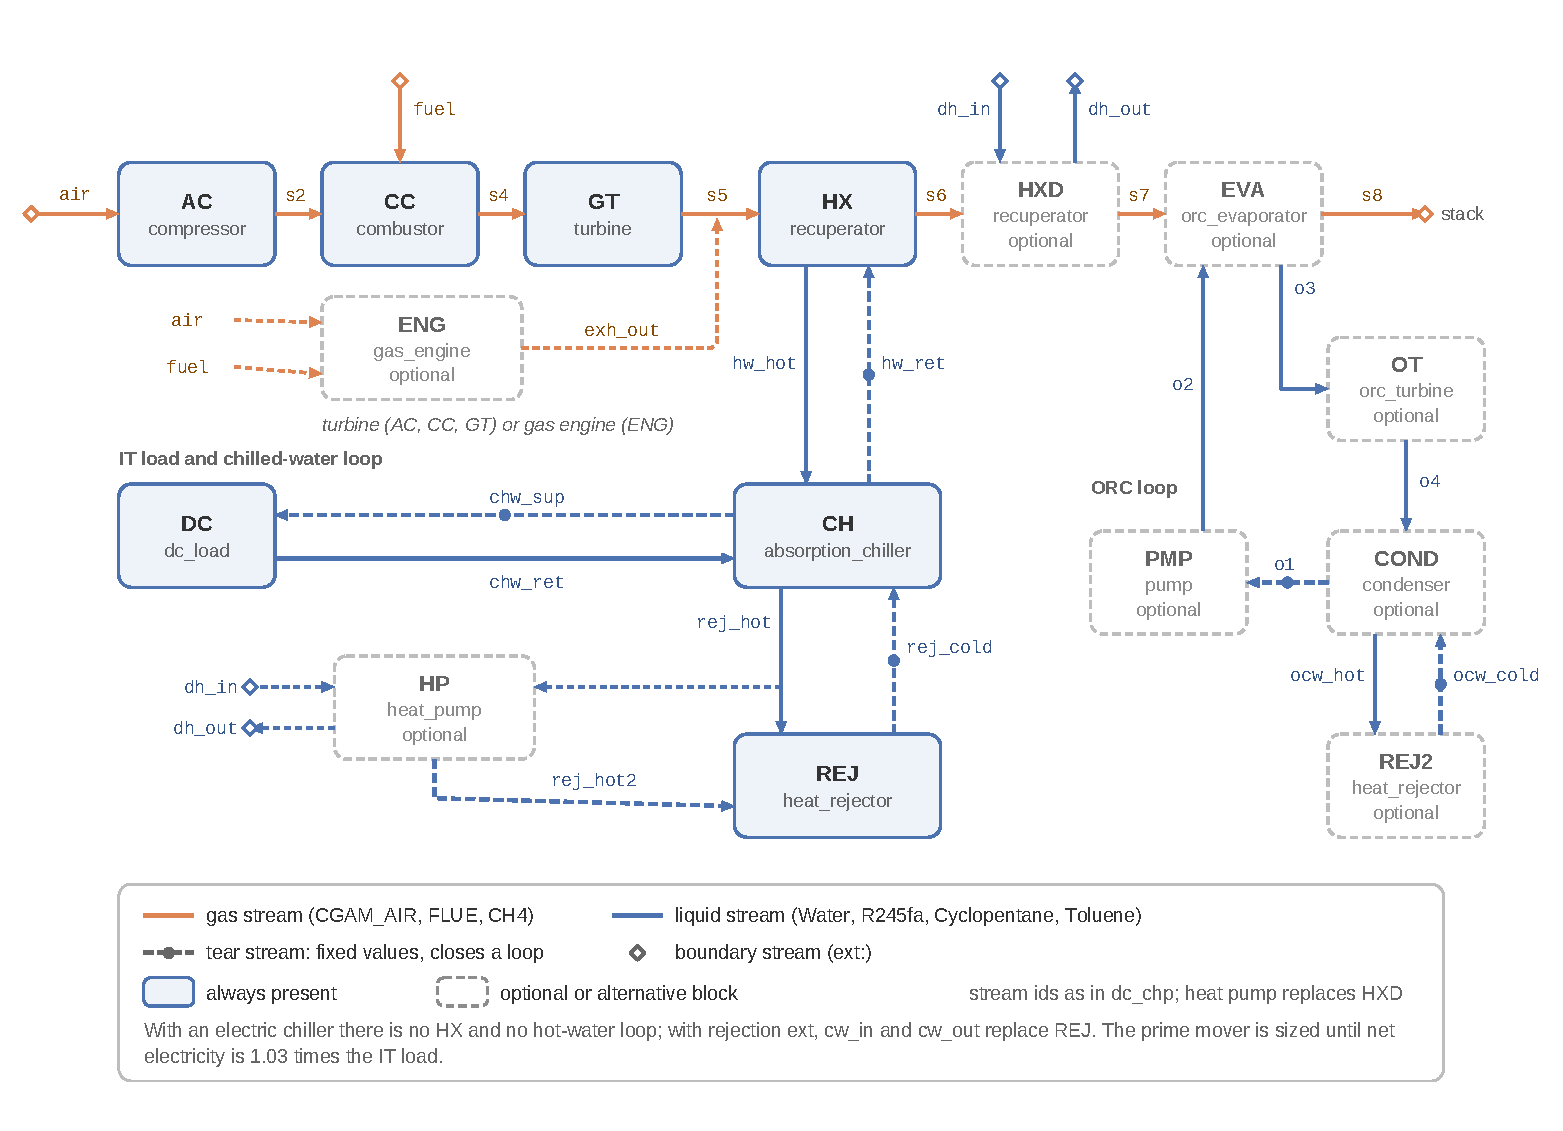
\includegraphics[width=\linewidth]{figures/pdf/fig_plant_graph.pdf}
\caption{Plant graph of the data-center model with the real stream identifiers. Gas streams are orange and liquid
streams blue; dashed streams are tear streams with fixed values that close a loop; dashed boxes are optional or
alternative blocks (gas engine, district-heat exchanger, ORC loop, second heat rejector, heat pump). The graph is
produced from three builder calls of the \texttt{dc\_chp} topology (\texttt{assets/plant\_graph.json}); it is a
structural diagram, not a result.}
\label{fig:fig_plant_graph}
\end{figure}

\paragraph{Component library.}
There are \val{env.n_components} component types with \val{env.n_params} registered parameters in total
(\cref{tab:components}; the full registry is in \cref{app:registry}). The main models are these. The combustor
solves a fuel-to-air mole ratio from an energy balance with a heat-loss fraction. The gas engine is sized by its
rated electrical output: fuel is $P_{\mathrm{el}}/(\eta_{\mathrm{el}}\,\mathrm{LHV})$, jacket and radiation heat
$f_{\mathrm{loss}}\,\dot n_F\,\mathrm{LHV}$ is rejected to ambient rather than recovered, and the exhaust
temperature follows from the balance. The absorption chiller has
$\mathrm{COP}=\min(\varepsilon\,\mathrm{COP}_{\mathrm{rev}},\mathrm{COP}_{\max})$ with $\varepsilon=0.27$ and a
cap of $0.8$, where $\mathrm{COP}_{\mathrm{rev}}$ is the reversible COP of the generator, rejection and
evaporator temperatures. Electric chillers and heat pumps use a fraction $\varepsilon=0.5$ of the reversible (Lorenz)
COP on refrigerant-side temperatures obtained by moving the stream log-mean temperatures outward by a 5~K approach.
The heat rejector's outlet is the dry-bulb temperature (dry cooler, 8~K approach) or the wet-bulb temperature (tower,
5~K approach) plus the approach; fans use 1.5\% of the heat rejected, and tower make-up water is an upper bound.
The ORC evaporator puts its pinch at the bubble point and lets the working-fluid flow lie in a window: the upper limit keeps the
exhaust above a stack floor of 333~K and the lower limit keeps the vapor at or below a fluid-specific temperature
(420, 480 and 560~K for R245fa, cyclopentane and toluene); if the lower limit exceeds the upper, the exhaust is too hot
for that fluid. The IT load consumes $P_{\mathrm{it}}$ of electricity and passes a fraction $f$ of it to a chilled-water
loop; the rest is rejected directly.

\begin{table}[tbp]
\centering
\begingroup\scriptsize\setlength{\tabcolsep}{4pt}\renewcommand{\arraystretch}{1.15}
\begin{tabular}{@{}p{3.2cm}p{4.9cm}p{7.0cm}@{}}
\toprule
Type & Ports (fluid class) & Parameters \\
\midrule
\texttt{compressor} & \texttt{in} (g), \texttt{out} (g) & \texttt{PR}, \texttt{eta\_s} \\
\texttt{turbine} & \texttt{in} (g), \texttt{out} (g) & \texttt{P\_out}, \texttt{eta\_s} \\
\texttt{orc\_turbine} & \texttt{in} (l), \texttt{out} (l) & \texttt{P\_out}, \texttt{eta\_s} \\
\texttt{pump} & \texttt{in} (l), \texttt{out} (l) & \texttt{P\_out}, \texttt{eta\_s} \\
\texttt{combustor} & \texttt{air\_in} (g), \texttt{fuel\_in} (g), \texttt{out} (g) & \texttt{T\_out}, \texttt{dp}, \texttt{q\_loss} \\
\texttt{recuperator} & \texttt{cold\_in} (?), \texttt{cold\_out} (?), \texttt{hot\_in} (?), \texttt{hot\_out} (?) & \texttt{T\_cold\_out}, \texttt{dp\_cold}, \texttt{dp\_hot}, \texttt{useful\_heat} \\
\texttt{hrsg} & \texttt{hot\_in} (g), \texttt{hot\_out} (g), \texttt{water\_in} (l), \texttt{steam\_out} (l) & \texttt{P\_steam}, \texttt{dp\_gas}, \texttt{econ\_approach\_K} \\
\texttt{orc\_evaporator} & \texttt{hot\_in} (g), \texttt{hot\_out} (g), \texttt{cold\_in} (l), \texttt{cold\_out} (l) & \texttt{pinch\_K}, \texttt{dp\_hot}, \texttt{flow\_frac}, \texttt{T\_stack\_min}, \texttt{T\_max\_K} \\
\texttt{condenser} & \texttt{hot\_in} (l), \texttt{hot\_out} (l), \texttt{cold\_in} (l), \texttt{cold\_out} (l) & \texttt{dT\_cw} \\
\texttt{dc\_load} & \texttt{in} (l), \texttt{out} (l) & \texttt{P\_it}, \texttt{chilled\_fraction}, \texttt{T\_return} \\
\texttt{absorption\_chiller} & \texttt{gen\_in} (l), \texttt{gen\_out} (l), \texttt{evap\_in} (l), \texttt{evap\_out} (l), \texttt{rej\_in} (l), \texttt{rej\_out} (l) & \texttt{T\_chw\_out}, \texttt{T\_gen\_out}, \texttt{dT\_rej}, \texttt{eps}, \texttt{COP\_max} \\
\texttt{heat\_pump} & \texttt{src\_in} (l), \texttt{src\_out} (l), \texttt{sink\_in} (l), \texttt{sink\_out} (l) & \texttt{T\_sink\_out}, \texttt{eps}, \texttt{approach\_K}, \texttt{Q\_sink}, \texttt{dT\_src} \\
\texttt{electric\_chiller} & \texttt{evap\_in} (l), \texttt{evap\_out} (l), \texttt{rej\_in} (l), \texttt{rej\_out} (l) & \texttt{T\_chw\_out}, \texttt{dT\_rej}, \texttt{eps}, \texttt{approach\_K} \\
\texttt{heat\_rejector} & \texttt{in} (l), \texttt{out} (l) & \texttt{kind}, \texttt{approach\_K}, \texttt{fan\_frac} \\
\texttt{gas\_engine} & \texttt{air\_in} (g), \texttt{fuel\_in} (g), \texttt{exh\_out} (g) & \texttt{P\_el}, \texttt{eta\_el}, \texttt{f\_loss}, \texttt{air\_excess}, \texttt{P\_exh} \\
\bottomrule
\end{tabular}\endgroup

\caption{Component library, generated from \texttt{core.components} (\texttt{REQUIRED\_PORTS},
\texttt{PORT\_CLASS}, \texttt{PARAMS}). Ports are marked g (gas) or l (liquid).}
\label{tab:components}
\end{table}

\paragraph{Sizing and topologies.}
The prime mover (the air flow of a turbine or the rated power of an engine) is scaled by secant iteration on full
plant solves until net electricity (generation minus parasitics plus ORC output) equals $1.03\,P_{\mathrm{it}}$. Two
topology families are used. The first is a gas turbine with an air preheater, an HRSG and an R245fa ORC, which is held
out as the steam-ORC topology. The second is the data-center plant \texttt{dc\_chp}: a prime mover (turbine or engine), cooling
(absorption or electric), heat rejection (an ideal boundary, a dry cooler or a wet tower), optional ORC bottoming with
one of three fluids, and optional district heat from the exhaust (a heat exchanger) or from a heat pump on the chiller
rejection water.

\paragraph{Cross-check.}
The generic engine was checked against an independent reference implementation of a gas turbine with an HRSG and an
R245fa ORC (one operating point, $n=1$). Net power agrees to \val{xchk.wnet_rel_pct}\%, energy efficiency to
\val{xchk.etaI_rel_pct}\%, and the HRSG pinch to \val{xchk.pinch_diff_K}~K; exergy closure holds to
\val{xchk.closure_w}~W, and component destruction agrees to \val{xchk.ed_max_rel_pct}\% or better. Exergy efficiency is
\val{xchk.etaII_diff_pct}\% (engine relative to reference), because chemical exergy is computed from the Gibbs energy of
the fuel reaction. This is a consistency check of the implementation, not a validation against a real plant.

\begin{table}[tbp]
\centering
\begingroup\small\renewcommand{\arraystretch}{1.12}
\begin{tabular}{@{}p{7.2cm}p{4.6cm}p{3.6cm}@{}}
\toprule
Constant (assumed, not fitted) & Code name & Default \\
\midrule
Compressor isentropic efficiency & \texttt{eta\_c} & 0.86 \\
Turbine isentropic efficiency & \texttt{eta\_t} & 0.88 \\
Pressure ratio & \texttt{PR} & 18 \\
Turbine inlet temperature (K) & \texttt{T4} & 1500 \\
Combustor pressure drop; heat loss fraction & \texttt{dp\_cc}, \texttt{q\_loss} & 0.04; 0.01 \\
Gas engine electrical efficiency & \texttt{eta\_el} & 0.43 \\
Gas engine loss fraction (jacket and radiation) & \texttt{f\_loss} & 0.15 \\
Air excess & \texttt{air\_excess} & 1.8 \\
Absorption chiller: fraction of reversible COP; COP cap & \texttt{eps\_abs}, \texttt{COP\_max} & 0.27; 0.8 \\
Electric chiller and heat pump: fraction of reversible COP & \texttt{eps\_ec}, \texttt{eps\_hp} & 0.5; 0.5 \\
Chilled-water supply and return (K) & \texttt{T\_supply}, \texttt{T\_return} & 291.15; 301.15 \\
Hot-water loop supply and return (K) & \texttt{T\_hw}, \texttt{T\_gen\_out} & 368.15; 358.15 \\
Rejector approach to ambient (dry or wet; K) & \texttt{dT\_rej} & 8 (dry), 5 (wet) \\
Rejector fan power (share of heat rejected) & \texttt{fan\_frac} & 0.015 \\
ORC working-fluid vapour limits (K) & \texttt{ORC\_T\_MAX} & R245fa 420; Cyclopentane 480; Toluene 560 \\
ORC condenser approach (K); pump and turbine efficiency & \texttt{orc\_cond\_approach}, \texttt{eta\_pump}, \texttt{eta\_orct} & 8; 0.75; 0.85 \\
Stack temperature floor for exhaust recovery (K) & \texttt{T\_stack\_min} & 333.15 \\
Fraction of the IT heat on the chilled-water loop & \texttt{chilled\_fraction} & 0.5 (Design: site input) \\
Sizing margin on net electricity & \texttt{margin} & 1.03 \\
\bottomrule
\end{tabular}\endgroup

\caption{Assumed technology constants with their code defaults (\texttt{synth/topologies.py}, \texttt{core.components}). They are model settings, not measurements.}
\label{tab:constants}
\end{table}

\subsection{Exergy accounting}\label{sec:exergy}

The dead state is $(T_0,P_0)$ with the ambient air composition. For a stream at $(T,P)$ the physical exergy per mole is
\begin{equation}
e_{\mathrm{ph}}=(h-h_0)-T_0\,(s-s_0),
\end{equation}
with $h_0,s_0$ evaluated at $(T_0,P_0)$ for the same composition. The chemical exergy of a gas mixture is
\begin{equation}
e_{\mathrm{ch}}=\sum_i y_i\,\varepsilon_i+R\,T_0\sum_i y_i\ln y_i,
\end{equation}
where $\varepsilon_i=-R\,T_0\ln y_{\mathrm{env},i}$ for the species present in the environment, so that ambient air has exactly
zero exergy, and $\varepsilon_{\mathrm{CH_4}}=-\Delta G+\varepsilon_{\mathrm{CO_2}}+2\varepsilon_{\mathrm{H_2O}}-2\varepsilon_{\mathrm{O_2}}$
with $\Delta G$ the Gibbs energy change of $\mathrm{CH_4}+2\,\mathrm{O_2}\rightarrow\mathrm{CO_2}+2\,\mathrm{H_2O(g)}$ at $(T_0,1~\mathrm{atm})$.
Liquids carry no chemical exergy. The exergy destruction of a component is
\begin{equation}
\ED=\sum_{\mathrm{in}}\dot n\,e-\sum_{\mathrm{out}}\dot n\,e-\dot W_{\mathrm{out}},
\end{equation}
and heat dissipated to the ambient carries no exergy. Over the plant,
$\sum\ED=\sum_{\text{ext. in}}\dot n\,e-\sum_{\text{ext. out}}\dot n\,e-\sum\dot W$ (closure), which holds to machine precision in the tests. The
exergy efficiency is
\begin{equation}
\eta_{\mathrm{II}}=\frac{\dot W_{\mathrm{net}}+\Delta\dot E_{\text{steam, heat, chilled water}}}{\dot E_{\mathrm{fuel}}}.
\end{equation}
\Cref{fig:fig_exergy_flow} shows one solved plant: a gas turbine with absorption cooling, a dry cooler and
district heat from the exhaust at a 20~MW IT load. Of \val{exf.fuel_mw}~MW of fuel exergy, \val{exf.cc_mw}~MW
(\val{exf.cc_share_pct}\%) is destroyed in the combustor, \val{exf.stack_mw}~MW leaves with the stack, and the delivered
cooling and heat carry only \val{exf.cool_ex_mw} and \val{exf.heat_ex_mw}~MW of exergy although they are
\val{exf.cool_mw} and \val{exf.heat_mw}~MW of energy. The heat rejector dissipates \val{exf.rej_energy_mw}~MW of energy
but destroys only \val{exf.rej_ed_mw}~MW of exergy, which is the contrast that \cref{sec:findings} measures over many plants.

\begin{figure}[tbp]
\centering
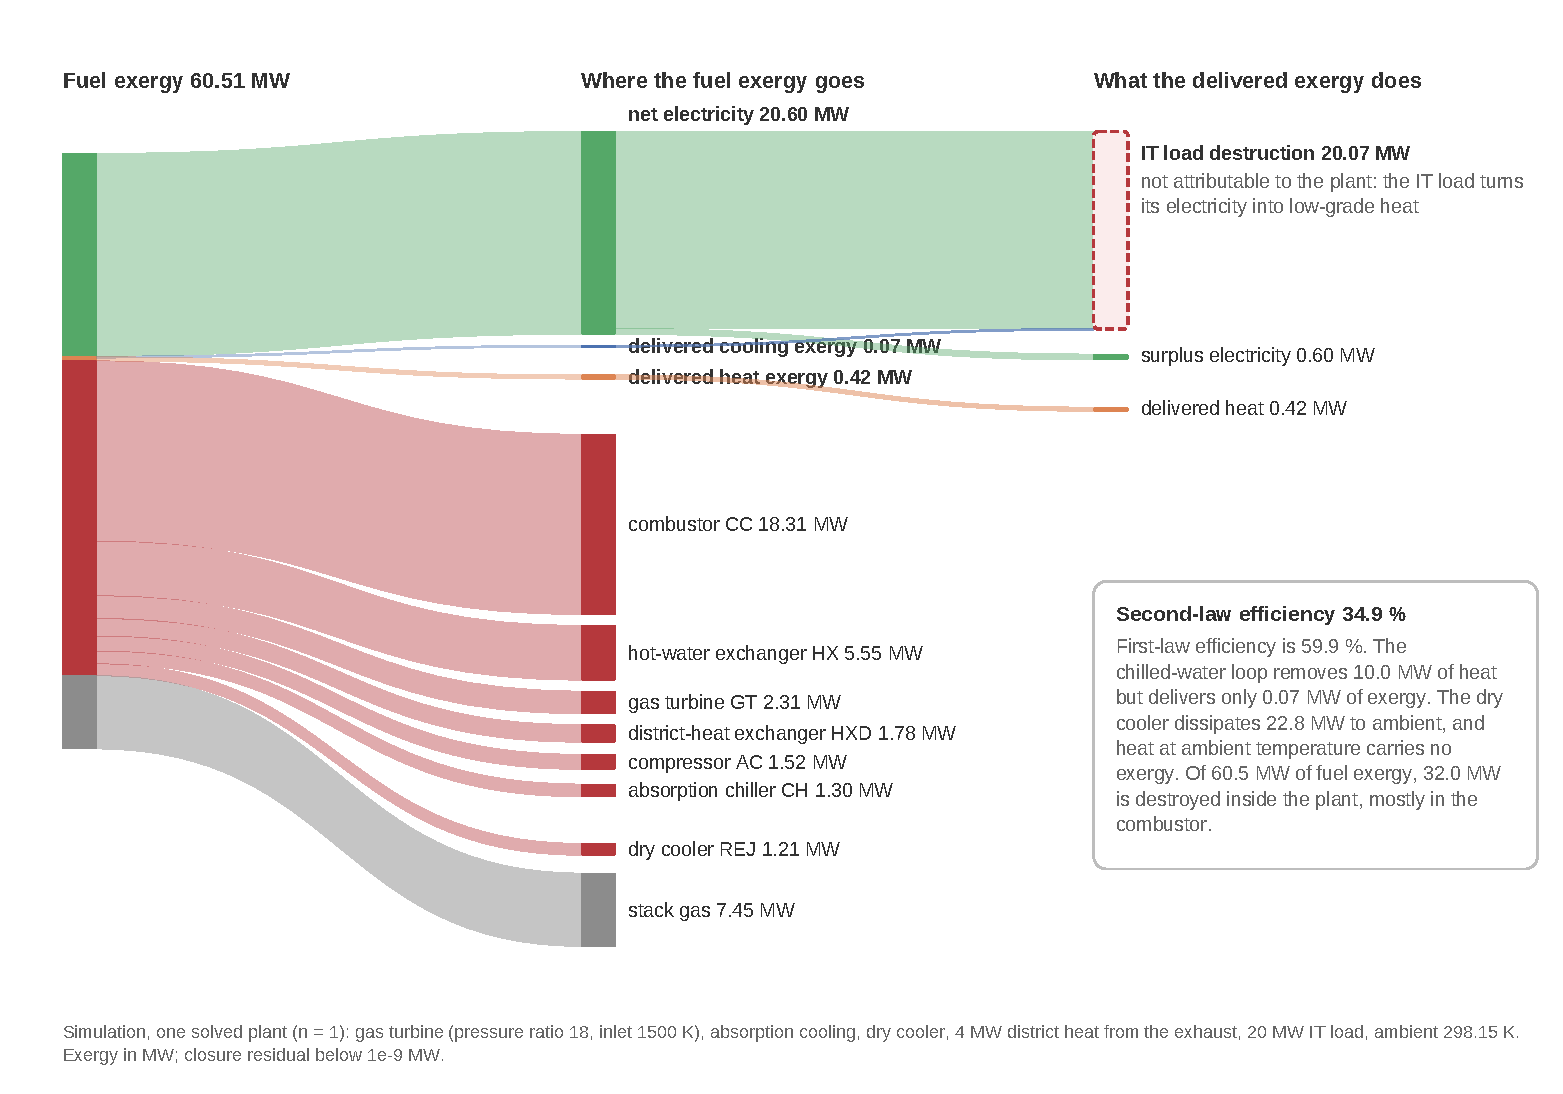
\includegraphics[width=\linewidth]{figures/pdf/fig_exergy_flow.pdf}
\caption{Exergy flow of one solved plant ($n=1$, simulation): gas turbine, absorption cooling, dry cooler, district heat
from the exhaust, 20~MW IT load. Ribbon widths are proportional to MW of exergy. Most fuel exergy is destroyed in the
combustor; cooling and heat are small in exergy terms; the destruction in the IT load itself
(\val{exf.dc_mw}~MW) is not attributable to the plant. Data: \texttt{assets/exergy\_flow.json}.}
\label{fig:fig_exergy_flow}
\end{figure}

\subsection{Verifiers}\label{sec:verifiers}

Eight verifiers decide whether a plant is acceptable (\cref{tab:verifiers}); the same checks are the reward
(\cref{sec:rewards}) and the feedback at inference. Hard checks gate validity; soft checks only lower a score.
V1 and V2 are balance checks. V3a requires non-negative destruction in every component, and V3b requires the closure
of \cref{sec:exergy}; together they are the second-law checks on the model itself. V4a rejects a temperature cross in any heat
exchanger, and V4b asks for a practical pinch of 1~K. V5 bounds the efficiencies and every COP by the reversible limit of its stream temperatures.
V6 holds parameter and state ranges and is what catches most parameter-level faults. V7 grounds the numbers in a model's reasoning text, and V8
checks that the plant serves the site.

\begin{table}[tbp]
\centering
\begingroup\small\renewcommand{\arraystretch}{1.15}
\begin{tabular}{@{}lp{3.3cm}p{7.6cm}p{1.9cm}@{}}
\toprule
ID & Check & Definition and tolerance & Kind \\
\midrule
V1 & mass balance & per component, residual $\le 10^{-6}$ of the largest flow & hard \\
V2 & energy balance & per component, residual $\le 10^{-6}\,(|\dot W_{\text{net}}|+\dot Q_{\text{fuel}}+1~\mathrm{MW})$ & hard \\
V3a & non-negative destruction & $\ED \ge -10^{-5}\,\dot E_{\text{fuel}}$ in every component & hard \\
V3b & exergy closure & $|\sum \ED - (\text{in} - \text{out} - \dot W_{\text{net}})| \le 10^{-6}\,\dot E_{\text{fuel}}$ & hard \\
V4a & temperature cross & minimum approach $\ge 0$ K in every heat exchanger & hard \\
V4b & practical pinch & minimum approach $\ge 1$ K & soft \\
V5 & second-law bounds & $0\le\eta_{\mathrm{II}}\le 1$; power efficiency $<1-\Tzero/T_{\max}$; ORC efficiency $<1-T_{\mathrm{cond}}/T_{\mathrm{hot}}$; every COP at or below its reversible limit & hard \\
V6 & parameter and state ranges & efficiencies in $(0,1]$, pressure ratio $>1$, drops in $[0,0.3]$, $T$ in 150--2500 K, $P$ in 1 kPa--100 MPa, pressure-change direction & hard \\
V7 & number grounding & numbers with units in reasoning text match solver or plant values within 0.5\% (3\% for predicted Design quantities) & reward channel \\
V8 & site requirements & IT load within 1\%, electricity balance (no grid import unless allowed), cooling and heat $\ge 99\%$, water limit & hard (site) \\
\bottomrule
\end{tabular}\endgroup

\caption{Verifiers V1 to V8 with tolerances. Hard checks gate validity.}
\label{tab:verifiers}
\end{table}

\begin{figure}[tbp]
\centering
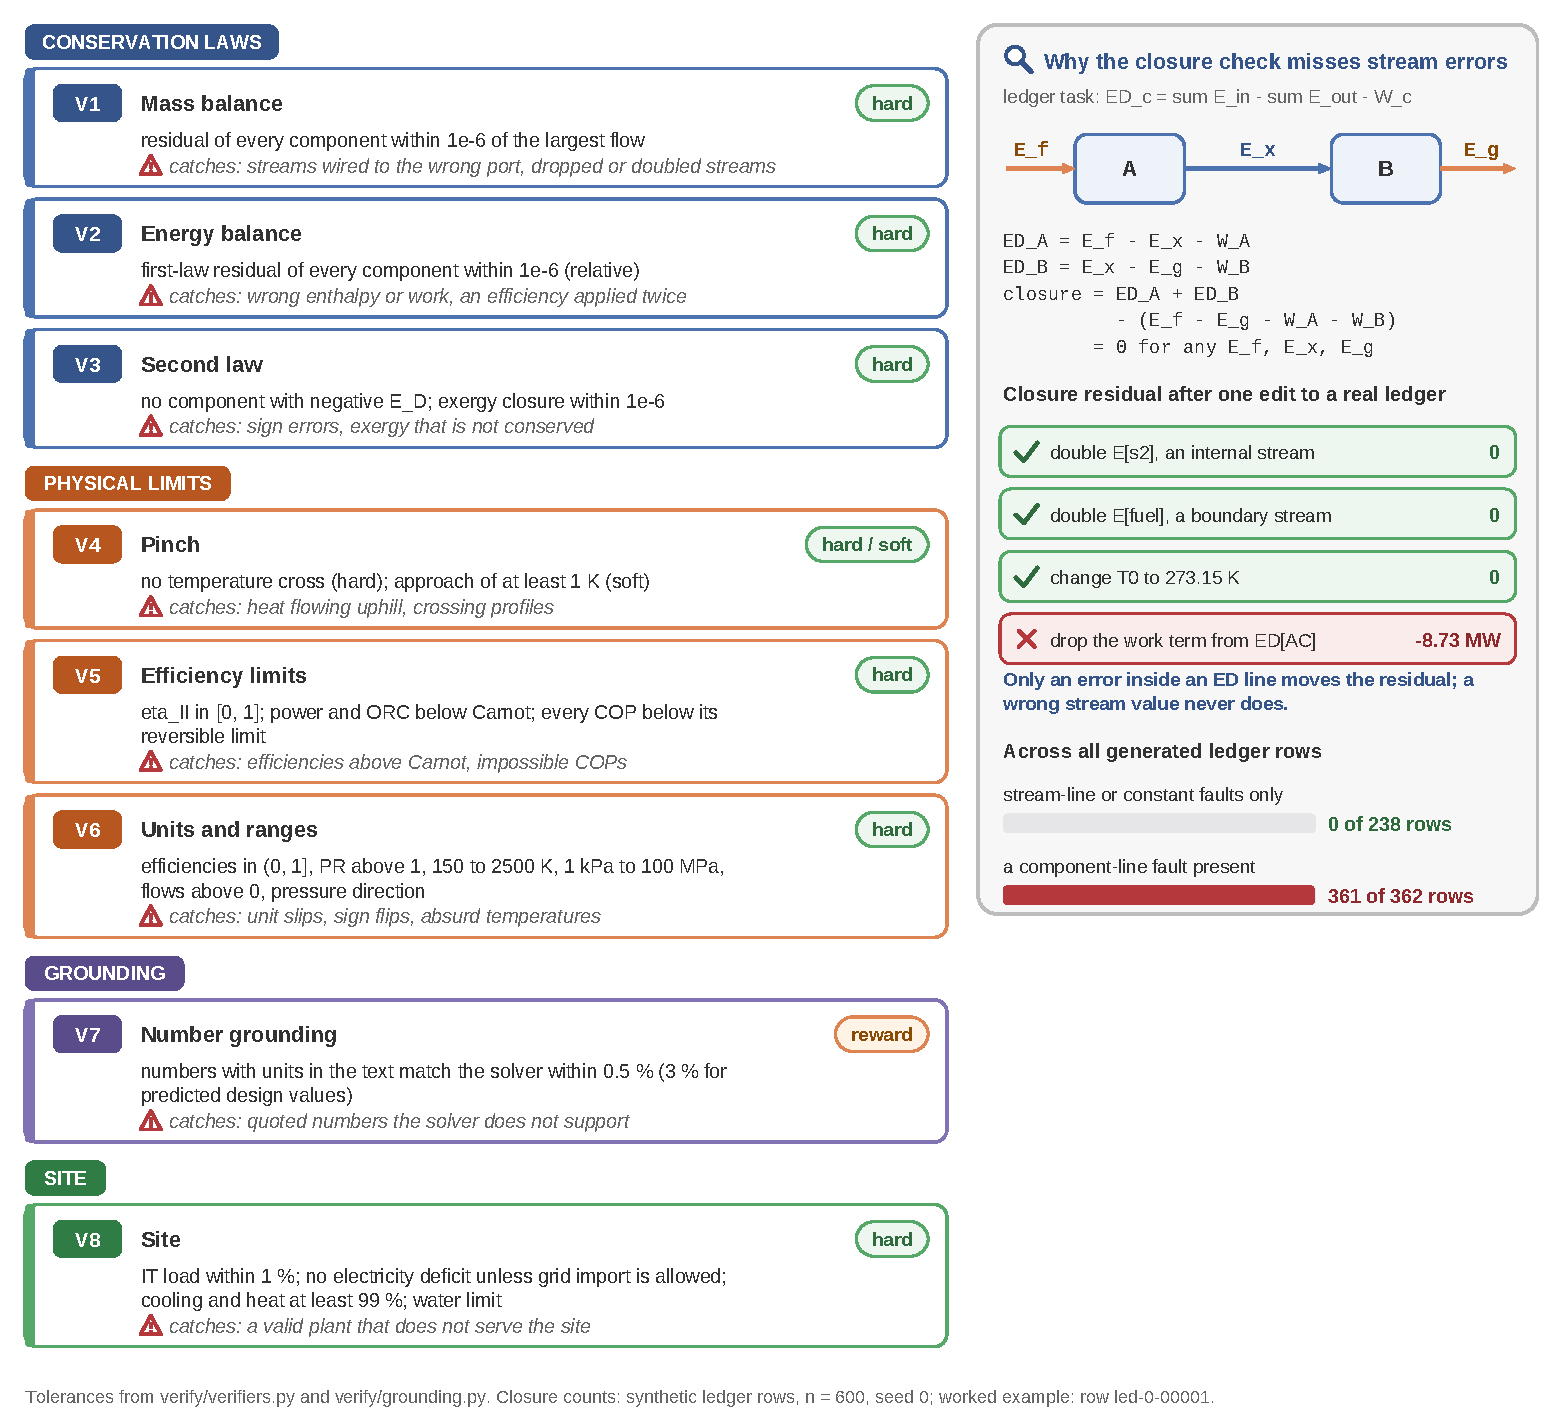
\includegraphics[width=\linewidth]{figures/pdf/fig_verifiers.pdf}
\caption{Verifiers V1 to V8 with tolerances and what each catches (left). Right: in the ledger task an error in any
stream value or in $T_0$ enters the closure sum with opposite signs and cancels; only errors in the destruction lines break
closure. The counts are from \val{led.n} generated ledger rows (seed 0, simulation): closure is broken in
\val{led.comp_closure} of \val{led.comp_rows} rows with a component-line fault and in \val{led.stream_closure} of
\val{led.stream_rows} rows with only stream-line or constant faults. Data: \texttt{assets/ledger\_symptoms.json}.}
\label{fig:fig_verifiers}
\end{figure}

\subsection{Tasks}\label{sec:tasks}

All four tasks are text in and text out. Plants are shown in a compact text language with one line per component
(\texttt{C id type \{params\}}) and per stream (\texttt{S id from -> to fluid \{extras\}}). \Cref{tab:tasks} summarizes the
tasks and \cref{fig:fig_tasks} shows verbatim excerpts of generated rows. The fault catalogs are in
\cref{app:faults}. Splits are structural: whole fault types, topologies or operating regimes are held out, and the rest
is split by a hash of the example identifier.

\begin{table}[tbp]
\centering
\begingroup\scriptsize\renewcommand{\arraystretch}{1.2}
\begin{tabular}{@{}p{1.5cm}p{3.2cm}p{2.8cm}p{3.3cm}p{3.3cm}@{}}
\toprule
Task & Input & Output & Reward channels (weight) & Held-out splits \\
\midrule
Repair & plant text, site, solver error or failed checks & \texttt{<diagnosis>}, at most 6 edits & format~0.5, valid~2, site~1, exact~1, minimal~0.5, grounded~0.5 & test ood fault: sign flip, swapped ports; test ood topology: 9 of 65 diagrams: the steam plant and the 8 gas-engine plants with ideal rejection \\
Design & site: IT load, chilled load, ambient $T$ and RH, coolant temperatures, optional heat demand and water limit & \texttt{<rationale>}, \texttt{<design>} block & format~0.5, valid~2, quality~2, grounded~0.5 & test ood scale: IT load of 45 MW or more; test ood climate: ambient 305 K or more; test ood load: chilled fraction 0.85 or more \\
Audit & solved plant with an energy-level summary & \texttt{<analysis>}, \texttt{<ranking>}, one \texttt{<change>}, \texttt{<prediction>} & format~0.5, rank~1.5, valid~1, gain~2, pred~1, grounded~0.5 & test ood topology: 9 of 65 diagrams: the steam plant and the 8 gas-engine plants with ideal rejection \\
Ledger repair & exergy ledger of a solved plant (arithmetic lines) & \texttt{<diagnosis>}, \texttt{FIX} lines & format~0.5, closure~1, nonneg~0.5, exact~2.5, minimal~0.5, grounded~0.5 & test ood fault: dropped\_work, wrong\_ref, wrong\_stream; test ood topology: 9 of 65 diagrams: the steam plant and the 8 gas-engine plants with ideal rejection \\
\bottomrule
\end{tabular}\endgroup

\caption{The four tasks: input, output, reward channels with weights (\cref{sec:rewards}) and held-out splits. Split
sizes are in \cref{app:datasets}.}
\label{tab:tasks}
\end{table}

\paragraph{Repair.}
A valid plant is broken by one of \val{env.n_repair_faults} fault types (unit slip, sign flip, efficiency above 1,
swapped ports, wrong fluid). The model reads the plant, the site and the solver or verifier output, and answers with
a diagnosis and at most six edits (\texttt{SET comp.param = x}, \texttt{SET @stream.field = x},
\texttt{REWIRE @stream.to = comp.port}, \texttt{FLUID @stream = fluid}) on existing numbers, endpoints and fluids. Every
injected fault that is kept is detected by the solver or the verifiers once the site specification is attached; most are
caught by range checks, which is why the Ledger task exists. The held-out splits are sign flip and swapped ports
(\texttt{test\_ood\_fault}) and the steam-ORC and gas-engine plants (\texttt{test\_ood\_topology}).

\paragraph{Design.}
The input is a site: IT load, chilled load, ambient temperature and humidity, coolant temperatures, and optionally a heat
demand and a water limit. The output is a \texttt{<rationale>} and a \texttt{<design>} block. The catalog combines prime mover
(turbine, engine), cooling (absorption, electric), rejection (dry, wet) and bottoming (none or an ORC on R245fa, cyclopentane
or toluene), which gives \val{env.n_catalog} configurations, doubled to \val{env.n_catalog_heat} by the heat source (exhaust or heat pump)
when there is a heat demand; seven continuous parameters (\texttt{dT\_rej}, \texttt{PR}, \texttt{T4}, \texttt{T\_hw}, \texttt{dT\_hw},
\texttt{P\_orc\_bar}, \texttt{orc\_frac}) complete a design. The objective is the least fuel among valid plants, with the services fixed by
the site. The reference is enumeration of the defaults followed by a Nelder--Mead polish of the best two; it is the best design found by this search, not a proven
optimum. Held-out regimes are an IT load of 45~MW or more, an ambient temperature of 305~K or more, and a chilled fraction of 0.85 or more.

\paragraph{Audit.}
The input is a solved plant with an energy-level summary; exergy destruction is hidden. The output is a ranking of exergy
destroyers, one allowed change (a set-point or loss parameter within $[0.8,1.25]$ of its value; component efficiencies and tear-closing temperatures
are excluded on purpose) and a prediction of the fuel change in MW after the prime mover is re-sized to the same net electricity.
The combustor or engine was the largest destroyer in every plant generated, so the ranking is scored with it removed.

\paragraph{Ledger repair.}
The exergy ledger of a solved plant is a list of arithmetic lines: \texttt{T0 = ...}; for every stream
\texttt{E[x] = m[x]*(h[x] - T0*s[x] - g0[x] + ech[x])/1e6}; for every component
\texttt{ED[c] = sum E[in] - sum E[out] - W[c]}. \val{env.n_ledger_faults} equation-level fault types in three layers
(stream lines, component lines, the constant) are injected into one or two lines; the model sees the ledger, the topology, the ambient
temperature, the stream values and the evaluated result, and answers with up to four corrected lines. Lines are evaluated by a
restricted arithmetic evaluator and nothing is executed. The held-out fault types are \texttt{wrong\_stream}, \texttt{dropped\_work} and
\texttt{wrong\_ref}. A program that rebuilds every line from the topology solves every row by construction, so the task measures whether a
model applies that rule from text and localizes the fault; this is a property of the benchmark, not an achievement of a model.

\begin{figure}[tbp]
\centering
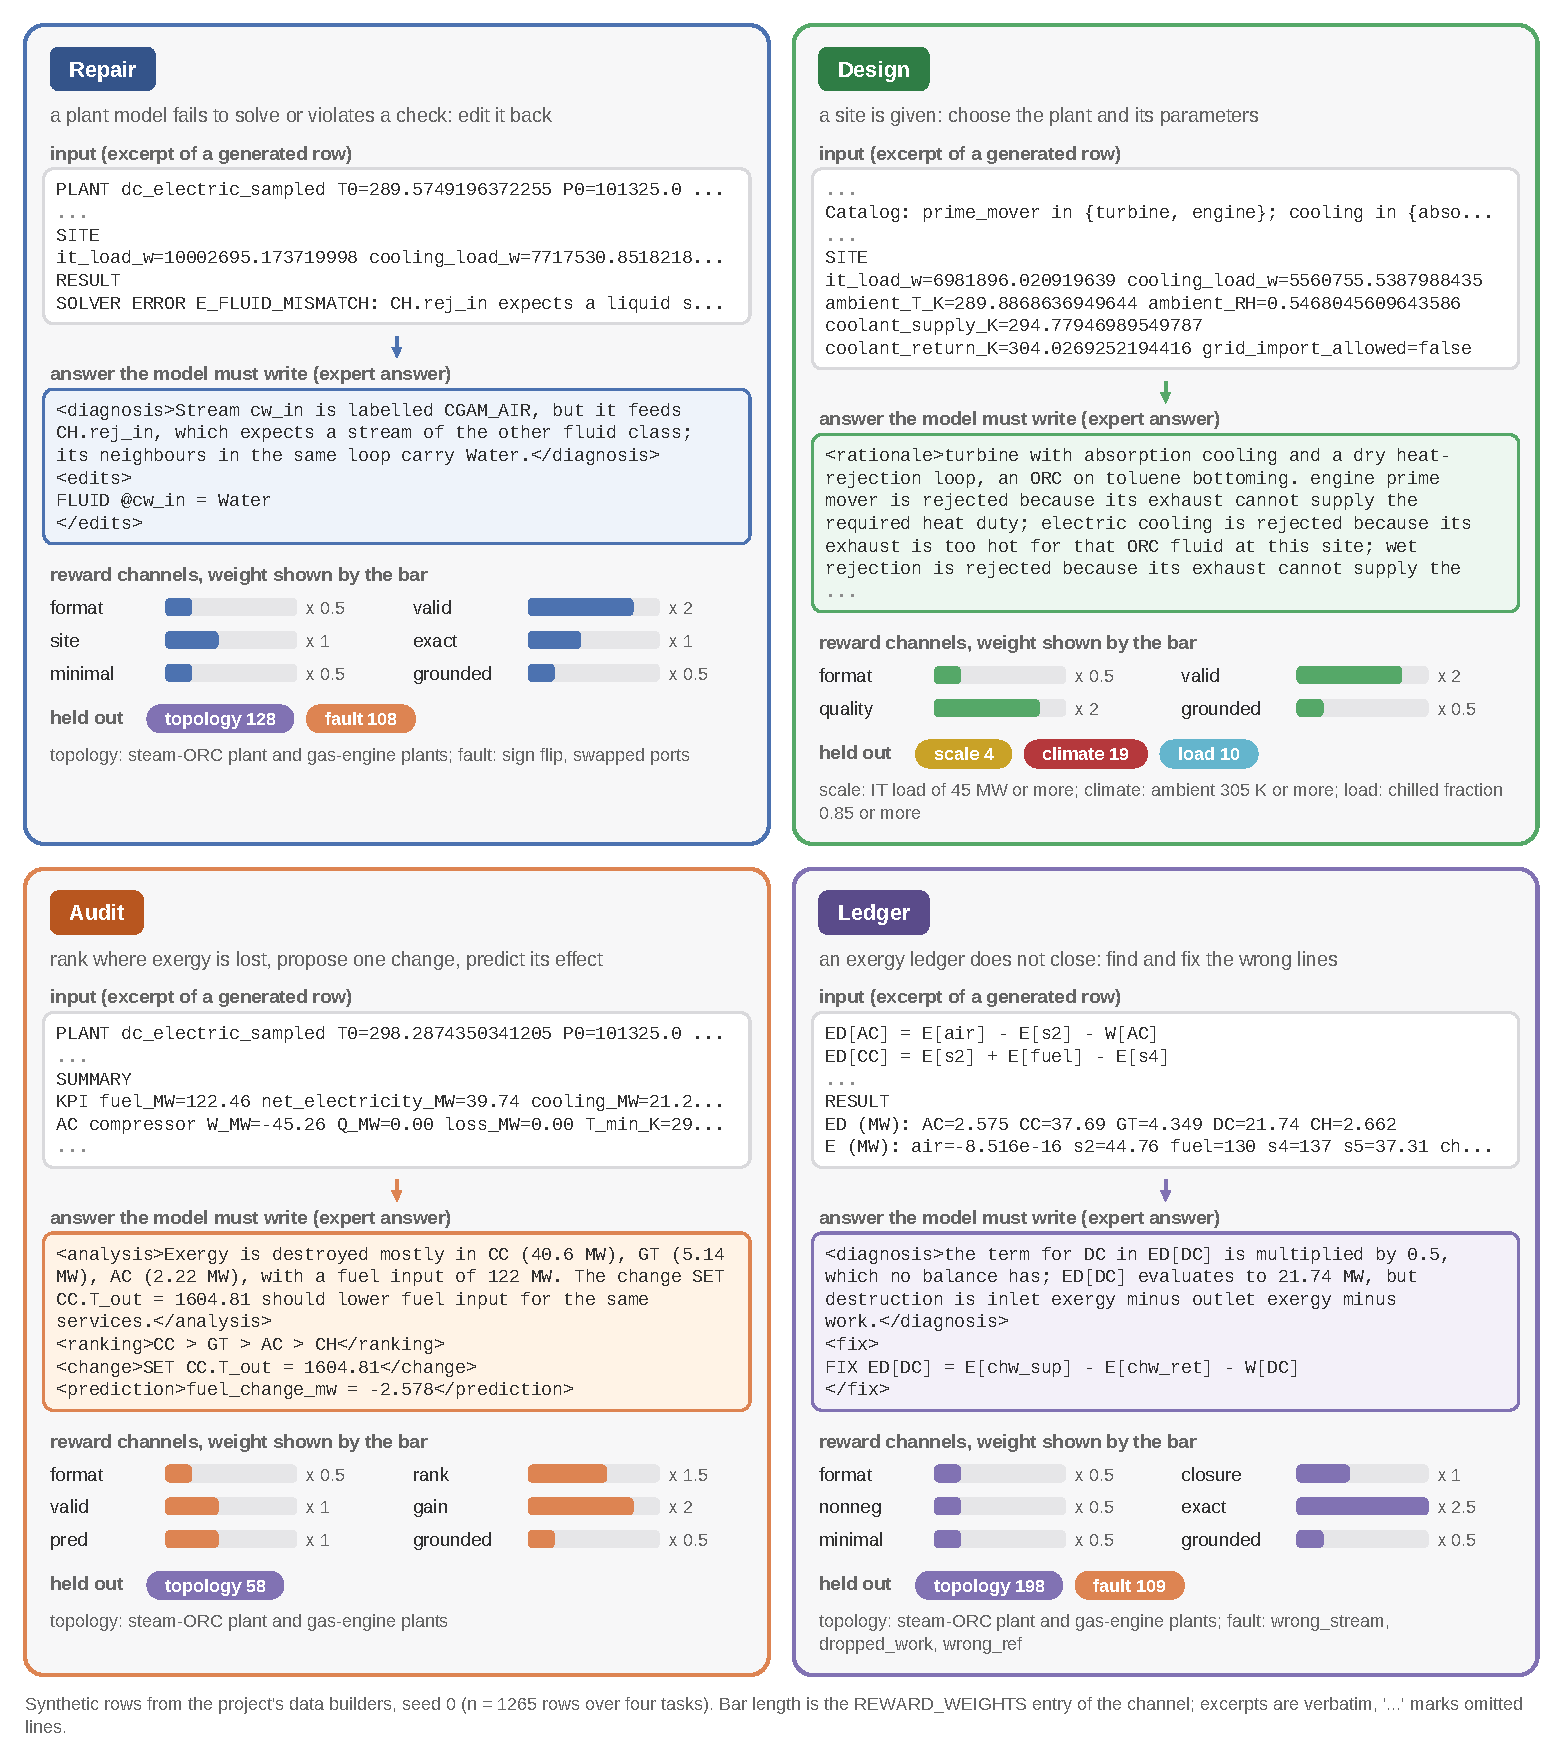
\includegraphics[width=\linewidth]{figures/pdf/fig_tasks.pdf}
\caption{The four tasks. For each: an excerpt of a generated input row, the expert answer the model must write, the reward
channels with their weights, and the held-out splits with row counts. Excerpts are verbatim from one generated training row
per task (seed 0; the row at the 12.5th length percentile); `\ldots' marks omitted lines. Data:
\texttt{assets/excerpts.json}, \texttt{assets/splits.json} (simulation, synthetic rows).}
\label{fig:fig_tasks}
\end{figure}

\subsection{Rewards}\label{sec:rewards}

Each task has its own channels; all are computed by the simulator and the verifiers, with no learned judge. Weights are in
\cref{tab:tasks}. \emph{Format} (0.5) rewards a parseable answer. \emph{Validity} (2 in Repair and Design, 1 in Audit) gives 1 if the plant
solves and passes every hard check and a partial credit otherwise (Repair: 0.5 times the fraction of checks passed; Design: 0.2 for a built but invalid plant).
\emph{Site} (1, Repair) requires the repaired plant to serve the site, so that deleting load is not a repair. \emph{Exact restoration} (1, Repair) applies only when the
original value is deducible from the broken plant. \emph{Minimality} rewards $1/(1+\text{extra edits})$. \emph{Quality} (2, Design) is
$1-(F-F_{\mathrm{ref}})/(0.1\,F_{\mathrm{ref}})$ clipped to $[0,1.05]$, so it is 1 at the reference fuel and 0 at 10\% more. In Audit, \emph{rank} (1.5) is nDCG@3 with the prime mover
removed, \emph{gain} (2) is the saved fuel divided by the best allowed saving, and \emph{prediction} (1) is
$1-|\hat y-y|/\max(|y|,0.002\,F)$. In Ledger repair, \emph{closure} (1) is 1 when the residual is within $10^{-6}$ of fuel exergy and falls to 0 at 1\%, \emph{non-negativity} (0.5) is the
share of components with $\ED\ge0$, and \emph{exactness} (2.5) counts faulty lines that now evaluate to the true value minus correct lines that are now broken. \emph{Grounding} (0.5) uses V7: every
number with a unit in the reasoning must match a solver or plant value.

Reward hacking is limited in three ways. Edits are restricted to existing fields, endpoints and fluids, so a model cannot add a component. The site check is part of the
Repair reward. The project's tests fuzz each reward function with junk and mutated answers and require that it never raises and stays bounded; this does not prove that
gaming is impossible, and we do not claim it.

\begin{figure}[tbp]
\centering
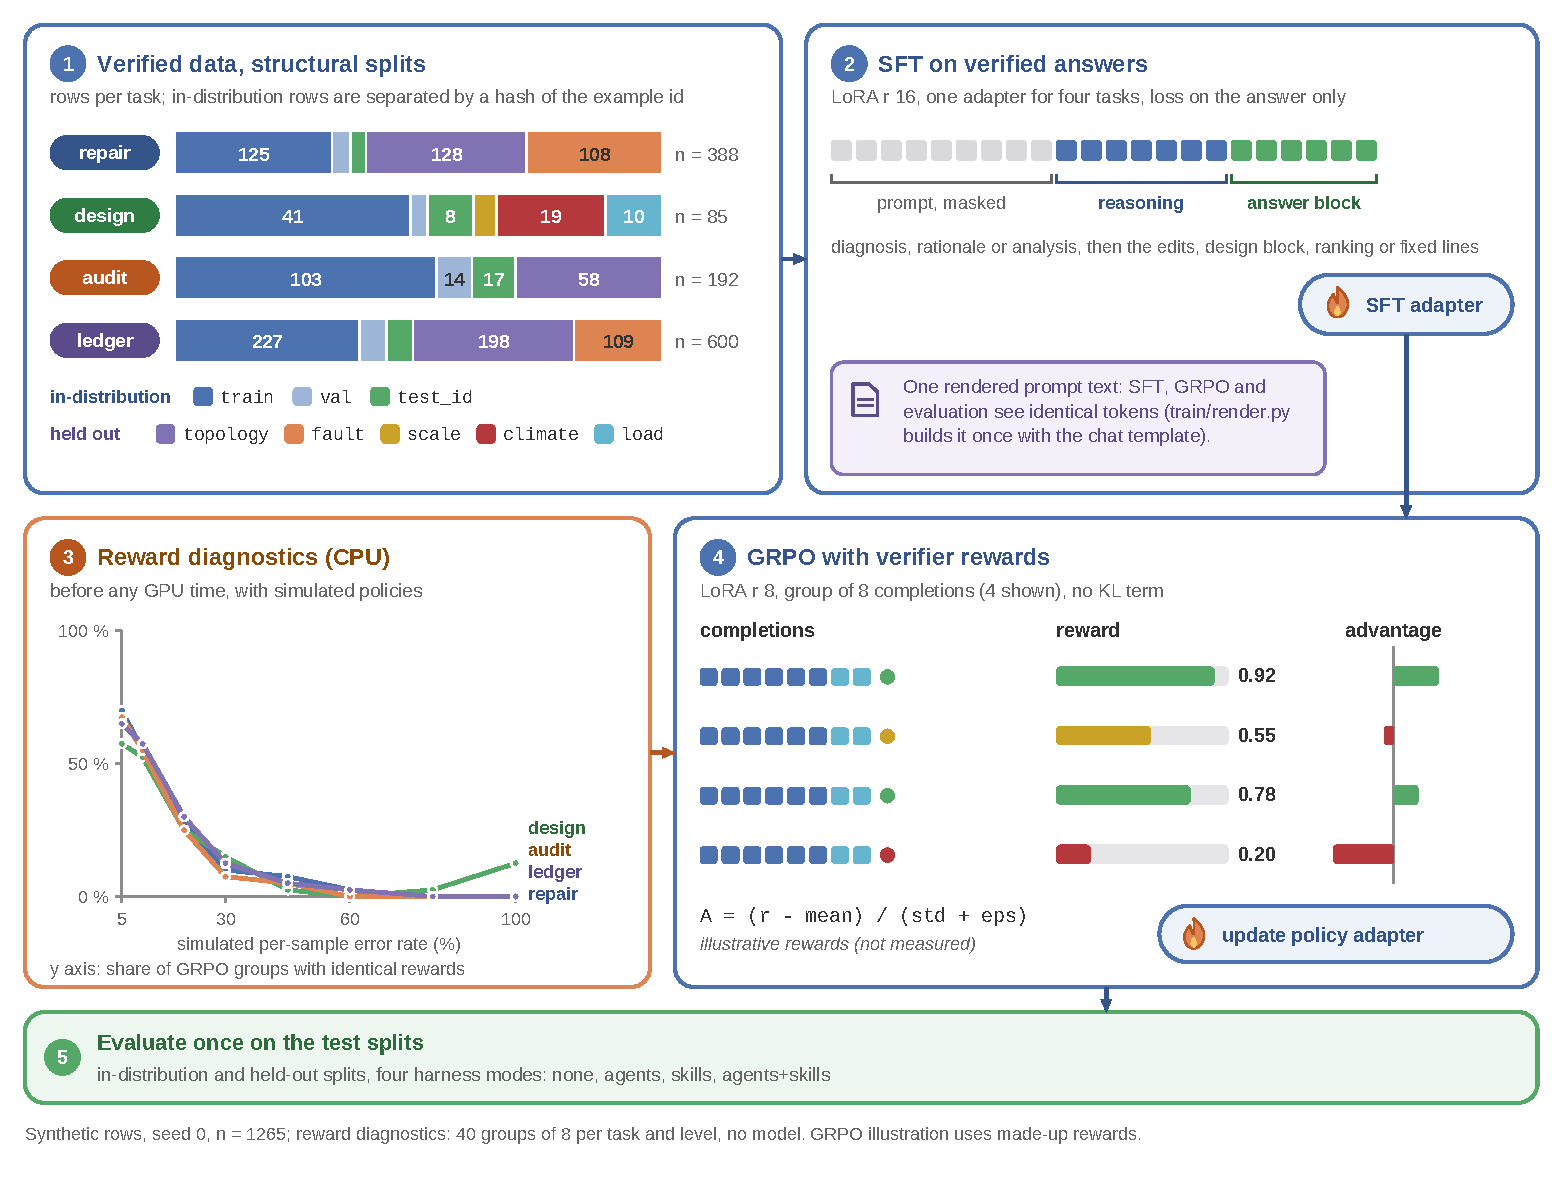
\includegraphics[width=\linewidth]{figures/pdf/fig_training.pdf}
\caption{Planned training pipeline and splits (pre-registered; no training has run). Tool rows use one compact harness and the plain A-slice uses the plain prompt; failure notes are added, prompts above \val{corp.max_prompt_chars} characters and \val{corp.max_prompt_tokens} tokens are dropped and counted (never truncated), and verifier-accepted frontier tool-using CoT traces are kept as SFT completions. The plan is SFT on two data-parallel ranks in fp16 with LoRA, merge, and one joint GRPO run with group sizes k = 4, 8 and 16 (distinct checkpoint paths, four prompts per step, $\mathrm{grad\_accum}=k$); reward diagnostics run on the CPU first, and evaluation is planned on the frozen \texttt{heldout\_v2} test set (the 214-id \texttt{heldout} is dev) over frontier zero-shot and harness replays, base 4B/9B, our SFT and GRPO k4/k8/k16, and other-LLM stand-in arms. Lower panel: rows per split of the ground-truth datasets (\val{split.total} rows from \texttt{data/processed} plus the diagram catalog \texttt{data/processed\_arch}, where \val{corp.arch_kept} of \val{corp.arch_requested} requested injections were kept). The decided corpus sizes are 4,800 tool rows per task family and a 1,600-row A-slice, both built; the remaining datagen item is the frontier chain-of-thought campaign (\cref{sec:datagenstatus}). Trained-model evaluation results are pending. Data: \texttt{assets/splits.json}, \texttt{assets/corpus.json} (simulation, synthetic rows).}
\label{fig:fig_training}
\end{figure}

\subsection{Training corpus}\label{sec:corpus}\label{sec:corpusstatus}

A model that sees one wording of one fault on one diagram can memorize it. The corpus therefore varies several axes at once, and every row is
accepted by the physics tool suite, not by its appearance. It has four sources, kept distinguishable by a source tag, plus the harness text (\cref{tab:corpus}). \Cref{fig:fig_corpus} shows the composition.

\paragraph{Current corpus status (datagen complete except frontier CoT).}
The corpus-side datagen is built and audited. The deterministic tool corpora hold 4,800 rows per task family (600 plants $\times$ 2 variants (direct, recover) $\times$ 4 tasks) with real physics tool results and 100\% verifier acceptance; the plain single-turn A-slice is complete at 1,600 rows ($=\mathrm{round}(4{,}800\times0.3333)$, 400 per task), held-out-excluded and re-measured with the real Qwen3.5 tokenizer. Every tool row is rendered with one compact harness text and the plain prompt is used only for the A-slice. Rows carry \texttt{easy}/\texttt{medium}/\texttt{hard} in equal thirds within each task, derived from the documented per-task size measure in \texttt{thermo\_agent/synth/tiers.py}, with the remainder to the higher tier and exact counts in the manifests. The test set \texttt{heldout\_v2} is frozen (3,476 scored rows in 12 cells, equal thirds per task, contamination scan PASS with zero overlap; \cref{sec:protocol}). Per-row provenance states deterministic vs AI and the exact model id on AI rows, and the token gate (8,192, measured with the real Qwen3.5 tokenizer) drops over-gate rows and counts them rather than truncating. The one open datagen item is the frontier harness chain-of-thought campaign (\cref{sec:datagenstatus}). No corpus has been used for training: no SFT step, GRPO step or checkpoint exists.

\begin{figure}[tbp]
\centering
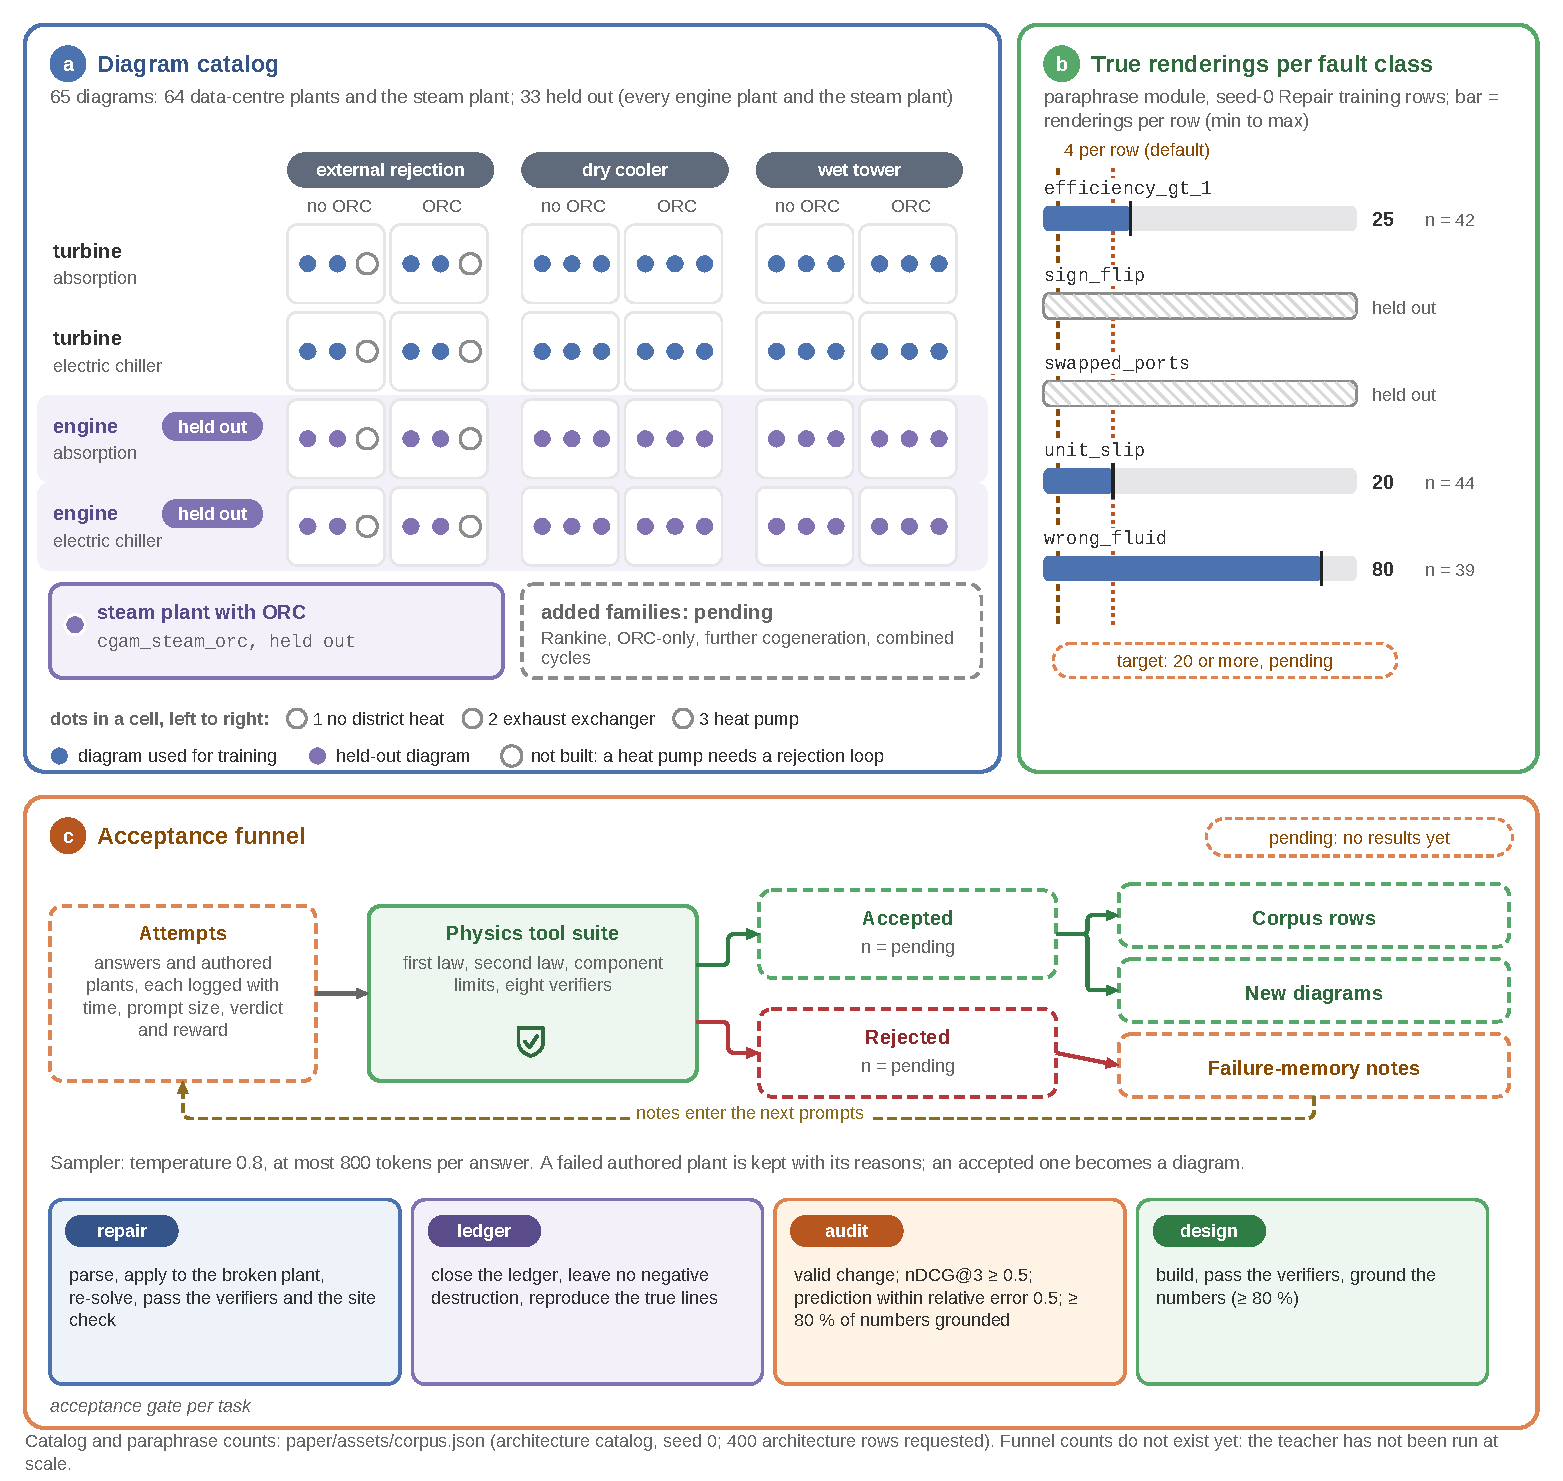
\includegraphics[width=\linewidth]{figures/pdf/fig_corpus.pdf}
\caption{Corpus composition. (a) The diagram catalog (\val{corp.n_arch} diagrams at the seed-0 sample): prime mover and cooling against rejection and ORC, with the district-heat options as dots; the \val{corp.n_held} held-out diagrams are the steam plant and the gas engines with the ideal-rejection boundary. (b) True renderings per fault class in the paraphrase module (\val{corp.var_min} to \val{corp.var_max}), with the held-out fault classes hatched. (c) The acceptance funnel from attempts through the physics tool suite to corpus rows, new diagrams and failure-memory notes, drawn as an empty skeleton: the teacher paths have not been run at scale. Data: \texttt{assets/corpus.json} (simulation).}
\label{fig:fig_corpus}
\end{figure}

\begin{table}[tbp]
\centering\small\renewcommand{\arraystretch}{1.15}
\begin{tabular}{@{}p{2.7cm}p{3.2cm}p{3.7cm}p{1.9cm}p{3.1cm}@{}}
\toprule
Source & Produced by & Gate & Varies & Role in training \\
\midrule
Ground truth with paraphrases & simulator and fault injectors & correct by construction (the original plant is restored) & wording & SFT rows with a fully known answer \\
Architecture corpus & catalog of labeled diagrams (\val{corp.n_arch} at the seed-0 sample) & the solver or the verifiers detect the injected fault & diagram & SFT rows on many system layouts; whole diagrams held out \\
Teacher answers & frontier models through Kaggle's model access & the physics tool suite accepts the answer & reasoning and edits & SFT rows with a second style of reasoning \\
Teacher-authored diagrams & the same models, writing plants in the plant language & the plant solves and passes the verifiers & diagram & new plants for the fault, ledger and audit rows \\
Hindsight memory & accepted and rejected attempts, compared with the ground-truth pattern & notes name a class of mistake or a working pattern, not the answer & what to recheck, and what passed before & success and failure notes in prompts at training and inference \\
Harness text & compact \texttt{AGENTS.md} and one selected skill & none & prompt text & one text for every tool row; plain prompt only for the A-slice \\
\bottomrule
\end{tabular}
\caption{Sources of the training corpus. The corpus builder combines them and records, per source, the rows kept and the prompts dropped.}
\label{tab:corpus}
\end{table}

\paragraph{Ground truth with paraphrases.}
Every Repair row is rendered from the injected fault and its inverse patch. For the seed-0 training rows, the paraphrase module has between \val{corp.var_min} and \val{corp.var_max} true renderings per fault class;
a row picks one by a hash of its identifier, and the corpus builder emits several per row (default \val{corp.variants_default}). Wording varies while the content cannot drift, because every rendering comes from the same facts.
The final corpus uses \val{corp.variants_default} variants per ground-truth Repair row, which is the whole pool of the sparsest fault class and a fifth of the largest, and the training split exercises \val{corp.var_max} distinct renderings across the classes. Ledger, Audit and Design rows vary through sampled plants, faults and sites, with one rendering each, because a paraphrase of a ledger row would only repeat the same site.

\paragraph{Architecture corpus.}
The catalog is a list of labeled plant diagrams: the data-center cogeneration plants (gas turbine or gas engine, absorption or electric cooling, ideal, dry or wet rejection, ORC bottoming on the remaining exhaust and district heat off the exhaust or a heat pump; a heat pump needs a rejection loop, so the eight combinations that lack one are skipped), and the steam-and-HRSG plant with an ORC, \texttt{cgam\_steam\_orc}.
At the seed-0 sample, the catalog has \val{corp.n_arch} diagrams, of which \val{corp.n_dc} are data-center plants; \val{corp.n_turbine} have a gas turbine and \val{corp.n_engine} a gas engine, \val{corp.n_orc} carry an ORC and \val{corp.n_heat} supply district heat.
Whole diagrams are held out, not single parameters: the eight gas-engine plants with the ideal-rejection boundary and the steam plant are in the held-out-topology split, so the model is tested on two layout combinations it never saw, while ORC, gas engines with dry or wet rejection, gas turbines and district heat all train.
The architecture generator was asked for \val{corp.arch_requested} fault injections over the catalog and kept \val{corp.arch_kept} (\val{corp.arch_kept_pct}\%) whose fault the solver or the verifiers detect; \val{corp.arch_distinct.train} distinct diagrams are in its training split and \val{corp.arch_distinct.test_ood_topology} in the held-out-topology split.

\paragraph{Teacher answers.}
Frontier models propose answers to the same prompts that the small model will see, with the harness text and retrieved memory notes in the prompt. They are reached through Kaggle's own model access (Kaggle Benchmarks and the Kaggle command line). The current campaign authorizes only \texttt{gpt-6-luna} and \texttt{claude-haiku-5-5}; each has completed a five-row proof (5/5 accepted) and one 100-row batch, with the journals at the local gate/ingest/audit stage. Luna uses a tools-without-reasoning setting (a documented deviation: the API rejects tools together with reasoning for luna). The target is thousands of verifier-accepted harness-CoT traces with no cap on traces, per-model counts, cost or rows, in equal thirds across \texttt{easy}/\texttt{medium}/\texttt{hard}; the old 72-cell premium target is discarded. Premium models (\texttt{gpt-6.2-sol}, \texttt{claude-sonnet-5-5}, \texttt{claude-opus-5-5-default}, \texttt{gemini-4-argon}) and \texttt{gemini-3.8-flash}/\texttt{gemini-3.5-flash-lite} are not to be run; no traces, costs or scores exist for them. Every file that reaches Kaggle goes through the private HF corpus repo \texttt{Reza-Nadimi/thermo-agent-corpora} into one Kaggle dataset: no local data is uploaded to Kaggle, credentials live only in the repository-root \texttt{.env}, and one generic notebook (\texttt{kaggle\_model\_runner.py}) serves every workflow. Prompts are exported to a file, run in a notebook, and the completions are downloaded and validated locally. An early, superseded pilot left a small number of legacy traces in the provenance ledger; they are not part of the current authorized luna/haiku campaign and no performance claim is made from them. For the current objective the frontier model runs inside a LangGraph harness where it can call the real physics tools, read numeric feedback and revise; a verifier-accepted trace is stored with its full reasoning, tool calls and revisions as the SFT completion, so the student learns tool use rather than only the final answer. The five exposed tools and their one-line contracts are: \texttt{inspect\_plant} --- solve / verify the plant or ledger as given, with no candidate argument; \texttt{first\_law\_check} --- mass / energy residuals (kg/s, W), convergence, tear residual and unit / range flags; \texttt{second\_law\_check} --- exergy destruction (MW), closure, non-negativity and Carnot / COP limits; \texttt{validity\_check} --- validity, failed checks, pinch approach and ranges; \texttt{solve\_plant} --- the full stream table ($T$, $P$, $h$, $s$, exergy). Grading / acceptance is deliberately not exposed as a tool (P0-8): the model receives only physics feedback and must decide for itself when its answer is acceptable.
The sampler records every attempt, accepted or not, with its timestamp, elapsed time, prompt size, verdict and reward, and a resumed run does not spend quota again on attempts already logged. Sampling is at temperature \val{corp.samp_temperature} with at most \val{corp.samp_max_tokens} tokens. The teacher never sees the ground truth.
An attempt becomes a training row only if the tool suite accepts it:
a Repair answer must parse, apply to the broken plant, re-solve and pass the verifiers and the site check; a Ledger answer must close the ledger, leave no negative destruction and reproduce the true lines;
an Audit answer needs a valid change, a ranking with nDCG@3 of at least \val{corp.ndcg_min}, a prediction within a relative error of \val{corp.pred_err_max}, and at least \val{corp.ground_min_pct}\% of the numbers in its analysis grounded in the plant; a Design answer must build, pass the verifiers and ground its numbers to the same share.
These checks are the verifiers of \cref{tab:verifiers}: balances, the first and second laws, the temperature cross in exchangers such as a preheater or an HRSG, and the limits on each component.
Attempts are not discarded. A rejected attempt becomes a failure note that names a class of mistake; an accepted attempt becomes a success note that names the working pattern and the edits that passed the verifiers. Both are retrievable, so the prompt carries what to avoid and what has worked.

\paragraph{Multi-turn tool-using trajectories.}
Training uses genuine multi-turn tool use for both teacher and student: the model reasons, emits a tool call, receives the real numeric result of a physics tool, reads it, revises, and calls again, for up to \texttt{DEFAULT\_MAX\_ROUNDS} = 6 rounds, before returning the final answer (decision D4 applies the same six rounds to trace generation, training and frontier H evaluation). A stored tool-using completion has the shape reason --- \texttt{<tool\_call>}/\texttt{<tool\_result>} pair --- revision --- another call, repeated, and always ends with the verifier-accepted answer; the frontier traces collected so far contain at most five assistant turns under the earlier harness, while the decided compact harness uses six. Tool results are environment output and never a training target: SFT masks every \texttt{<tool\_result>} span and the Qwen-native \texttt{<tool\_response>} form, tags included, to $-100$, while reasoning, calls and the final answer stay trainable. A row is tagged as tool-using only when its stored completion actually contains tool turns; a harness record with no calls is not relabelled just because it carried a trajectory.

\paragraph{Teacher-authored diagrams.}
The teacher is also asked to write whole plants in the plant language, for a stated purpose such as a cogeneration plant for a given site or a Rankine cycle with a given steam condition. The solver and the verifiers check each plant: it must solve, close every balance, show no temperature cross
and keep every component inside its limits, and a plant that fails is kept with its reasons. An accepted plant becomes a new diagram. The fault injectors, the ledger program and the audit procedure then turn it into Repair, Ledger and Audit rows with a known answer, and the teacher can be sampled on those rows in turn. The model therefore reads diagrams that the catalog builders did not write
(none have been accepted at the time of writing, so this share is currently empty).

\paragraph{Hindsight success-and-failure memory.}
Each rejected attempt becomes a short note: the task, the fault class, the diagram, the symptom that the verifiers reported, the class of the mistake and the correct pattern from the ground truth. Notes are retrieved by lexical token overlap with the current plant text,
with a small boost when the query names the note's fault class or diagram, a minimum score of \val{corp.mem_min_score} and a limit of \val{corp.k_memory} notes, and any note mined from the same record is excluded. Notes describe classes of mistakes and never the answer to the current row;
they are appended after the harness text so that the model reads the usual failure modes for a plant of this kind and rechecks its answer. The sampler writes new notes into a shared memory directory, so the next prompt and the student read them. The retrieval is lexical and not an embedding search. A check that notes mined from training records cannot leak information into a held-out split is planned and has not yet passed.

\paragraph{Compact served memory.}
The ledger on disk is for our analysis; what is served to the model is a short recap, one line per retrieved note, each marked \texttt{OK} (verifier-accepted) or \texttt{FAIL} (verifier-rejected) and pairing a fault class with a reusable fix pattern. Bookkeeping is deliberately dropped before prompting: model and provider identifiers, timestamps, cost, token counts, latency, record identifiers, architecture and the raw checker log do not reach the model. Hand-written seed method notes (\texttt{source: seed:method}) are capped to at most one per served block, with the freed slots backfilled by verifier-mined notes, so generic guidance cannot crowd out plant-specific evidence. For one representative repair query at $k=3$, the rendered block measured 159 tokens with the Qwen3.5-4B tokenizer (76 words).

\paragraph{Combination.}
The corpus builder merges the sources into one file per task and split, renders every tool row with the compact harness and leaves the plain A-slice in its plain single-turn form, adds retrieved notes, and measures every prompt with the model's own tokenizer, dropping rows above \val{corp.max_prompt_chars} characters or \val{corp.max_prompt_tokens} tokens so that no row is silently truncated to fit the sequence length. It writes a report of dropped prompts, rows per source and a check of the expert reward. A second pass re-reads the written files, compares every row count with that report and checks that no identifier crosses a split, so a corpus that was moved or half-copied fails before training starts.
The ground-truth source corpus has \val{corp.rows} rows, \val{corp.rows_train} of them in the training split: Repair \val{corp.rows.repair.train}, Ledger \val{corp.rows.ledger.train}, Audit \val{corp.rows.audit.train} and Design \val{corp.rows.design.train}. The decided training mix (\texttt{sft\_mix\_h}) is the 4,800-row deterministic tool corpus plus the 1,600-row plain A-slice, with verifier-accepted frontier traces added first as they arrive. The teacher-authored share is empty at the time of writing: frontier harness-CoT datagen is still in progress (luna and haiku proofs plus one 100-row batch each) and has yielded accepted tool traces, not a corpus of teacher-authored diagrams.

\paragraph{Provenance.}
Every training row must state whether it is deterministic or AI-generated, and if AI-generated which model produced it. Deterministic rows are derived from ground truth by the simulator and the fault injectors, not written by a language model; frontier rows carry the exact model id and journal path. This tag is part of the row schema and is checked before a corpus is accepted.

\begin{table}[tbp]
\centering
\begingroup\small\renewcommand{\arraystretch}{1.15}
\begin{tabular}{@{}p{2.3cm}p{2.6cm}p{2.6cm}p{3.1cm}p{3.1cm}@{}}
\toprule
Task & Teacher attempts & Accepted (share) & Rejected, kept as notes & Distinct architectures accepted \\
\midrule
Repair & \todo{pending} & \todo{pending} & \todo{pending} & \todo{pending} \\
Ledger repair & \todo{pending} & \todo{pending} & \todo{pending} & \todo{pending} \\
Audit & \todo{pending} & \todo{pending} & \todo{pending} & \todo{pending} \\
Design & \todo{pending} & \todo{pending} & \todo{pending} & \todo{pending} \\
\bottomrule
\end{tabular}\endgroup

\caption{Teacher acceptance statistics, to be filled once the campaign completes. Frontier harness-CoT datagen is in progress with two authorized budget models (a five-row proof and one 100-row batch each); no model has been trained or evaluated, so the campaign-wide cells remain pending.}
\label{tab:corpusstatus}
\end{table}

\subsection{Training}\label{sec:training}

\paragraph{Stage 1: supervised fine-tuning.}
Qwen3.5-4B is fine-tuned with LoRA on the combined corpus of \cref{sec:corpus}, with one adapter for all four tasks. Thinking is enabled (\texttt{enable\_thinking=True}) in training, GRPO and evaluation. Prompts are rendered identically in all three, as plain prompt and completion text, so that no template mismatch arises between training and
inference. Supervised fine-tuning comes first because verifiable rewards are sparse for a policy that never succeeds \citep{lambert2024tulu3}. The maximum length is \val{tr.sft_len} tokens, and a prompt that is too long is dropped and counted, never truncated.
The planned SFT settings (decisions A1--A10, B1--B7) are learning rate $10^{-4}$, at most three epochs with early stopping after three evaluations without validation-loss improvement (best checkpoint loaded at the end), a cosine schedule with warmup ratio 0.05, weight decay 0, AdamW, seed 0, gradient clipping 1.0, LoRA rank 32 / alpha 64 / dropout 0.05 on all linear layers in float16, an effective batch of $2\times8\times2=32$ sequences per step, and save/evaluate every 50 steps. The training corpus is the \texttt{sft\_mix\_h} mix of the plain A-slice and the compact-harness tool rows. None of this has been run.

\paragraph{Stage 2: GRPO.}
The best SFT adapter is merged, and one joint GRPO run over all four tasks starts from the merged policy (\texttt{runs/sft\_merged}) with a new rank-8 / alpha-16 LoRA adapter. Completion sampling uses temperature 1.0, top-p 1.0, top-k off, no penalties, and beta 0 (no reference model); the loss is DAPO \citep{yu2025dapo} with group-normalized rewards and truncated completions masked. The reward is the weighted channel sum of \cref{tab:tasks}, dispatched by each prompt's task; prompts are sampled uniformly over task by tier. The maximum completion length is 4,096 tokens for the whole multi-turn completion, with at most six tool-calling iterations; a 320-token budget cannot hold a tool trace, and if dev truncation exceeds 10\% the limit is raised to 6,144. We plan group sizes $k\in\{4,8,16\}$ with four prompts per optimizer step, so $\mathrm{grad\_accum}=k$ on two GPUs (16, 32 and 64 sequences per step); all three use the same step count and seed 0. Zero-variance groups are logged, and the run stops if their share exceeds 50\% for ten consecutive logs. These settings (decisions C1--C10) are planned and have not been run.

\paragraph{Data parallelism.}
Training targets two T4 GPUs on one host, joined by PCIe without NVLink. The base model is replicated on each GPU (distributed data parallel), so that only the LoRA gradients, tens of megabytes in fp16, cross the link, once per optimizer step; sharding the 4B weights would move about 8~GB per step over the same link.
The T4 has no bf16 kernels, so the model runs in fp16 with dynamic loss scaling, gradient clipping and fp32 accumulation in matmuls, and 4-bit weights are not used. The effective batch is \val{tr.sft_batch_eff} sequences for SFT and \val{tr.grpo_batch_eff} prompts of \val{tr.group} completions for GRPO (\cref{tab:training}).
The code is written against TRL \citep{vonwerra2020trl} and has not been run on a GPU; loading the model, the library's argument names, fp16 overflow, merging and generation-length cutoffs are the known risks.

\begin{table}[tbp]
\centering
\begingroup\small\renewcommand{\arraystretch}{1.12}
\begin{tabular}{@{}p{4.2cm}p{5.4cm}p{5.6cm}@{}}
\toprule
 & Stage 1: SFT & Stage 2: GRPO \\
\midrule
Base model & \texttt{Qwen/Qwen3.5-4B} & \texttt{Qwen/Qwen3.5-4B} \\
Method & LoRA SFT, all tasks in one adapter & GRPO per task on the merged SFT model \\
Precision and parallelism & fp16 LoRA, DDP over 2 ranks (2 T4), no 4-bit & fp16 LoRA, DDP over 2 ranks, no 4-bit \\
LoRA rank / alpha / dropout & 16 / 32 / 0.05 & 8 / 16 / 0.05 \\
Target modules & all-linear & all-linear \\
Learning rate & 0.0002 & 5e-05 \\
Epochs or steps & 2 epochs & 300 steps (maximum) \\
Maximum length (tokens) & 4096 & completion 320 \\
Batch per device / accumulation / ranks & 2 / 8 / 2 & 4 / 2 / 2 \\
Effective batch & 32 sequences & 16 prompts, 4 completions each \\
Group size / temperature & -- & 4 / 1 \\
Gradient clipping & max norm 1 & max norm 1 \\
Loss & causal LM, completion tokens only & dapo-style, KL coefficient 0, truncated completions masked \\
Prompt rendering & tokenizer generation prompt, thinking disabled & same text as SFT and evaluation \\
\bottomrule
\end{tabular}\endgroup

\caption{Training settings, read from \texttt{train/config.py} (ranks from the dual-T4 recipe of the repository). None of this has been run on a GPU.}
\label{tab:training}
\end{table}

\paragraph{Reward diagnostics.}
Before any GPU time, each reward is probed with simulated policies that return the expert answer with probability $1-e$ and a damaged answer otherwise. For groups of
\val{rd.G} completions the diagnostic reports the share of groups whose rewards are all equal; the training group is \val{tr.group}, so the diagnostic is run at that size and, for comparison, at 8, where equal groups are less frequent. Such groups carry no gradient under group-normalized advantages, so they indicate the error rate below
which GRPO stops being informative for a task (\cref{sec:rewarddiag}).

\subsection{Agent harness and memory}\label{sec:harness}

The harness is text added to the system message. An \texttt{AGENTS.md} file holds conventions, verifier meanings, how to read solver errors and the answer formats; \val{env.n_skills} skills cover the gas
engine, heat rejector, absorption chiller, ORC bottoming, heat pump and district heat, the exergy audit, the design catalog and the exergy ledger. The port and parameter sections of the
skills are generated from the component registry, and a test fails if they drift from it. There are four harness modes: none, \texttt{AGENTS.md}, skills, and both. In the skill modes the bodies of the selected skills
are appended to the system message (they are not loaded on demand); a component skill is selected when its component appears in the plant. When there is no plant yet, as in Design, only the task's own skill (the design catalog, which lists the components and their parameters) is given, because every component skill at once would push a Design or Ledger prompt past the length limit.
The hindsight memory (\cref{sec:corpus}) is a separate layer that can be switched on independently of the mode, in the SFT prompts, in the GRPO rollouts and in evaluation, so that the harness ablation stays a four-mode comparison and memory adds a second factor.
The planned ablation holds the gas engine out of the training diagrams, so that its skill is its only description (\cref{sec:experiments}).

\paragraph{Compact harness.}
For every arm --- trace generation, training and frontier H evaluation --- the harness is one compact text of at most 2,500 tokens measured with the real Qwen3.5 tokenizer (decisions J2/J3): it keeps the tool contract, output tags, the failure checklist and the one selected skill, and drops prose examples and non-selected skills. The sequence gate stays at 8,192 tokens; over-gate rows are dropped and counted, never truncated. The harness runs six tool rounds with a memory limit of $k=3$ notes (decisions D4/D5). The compact harness text is built, audited and used for the frontier CoT traces; no training or evaluation arm has been run under any harness and no checkpoint exists.

\begin{figure}[tbp]
\centering
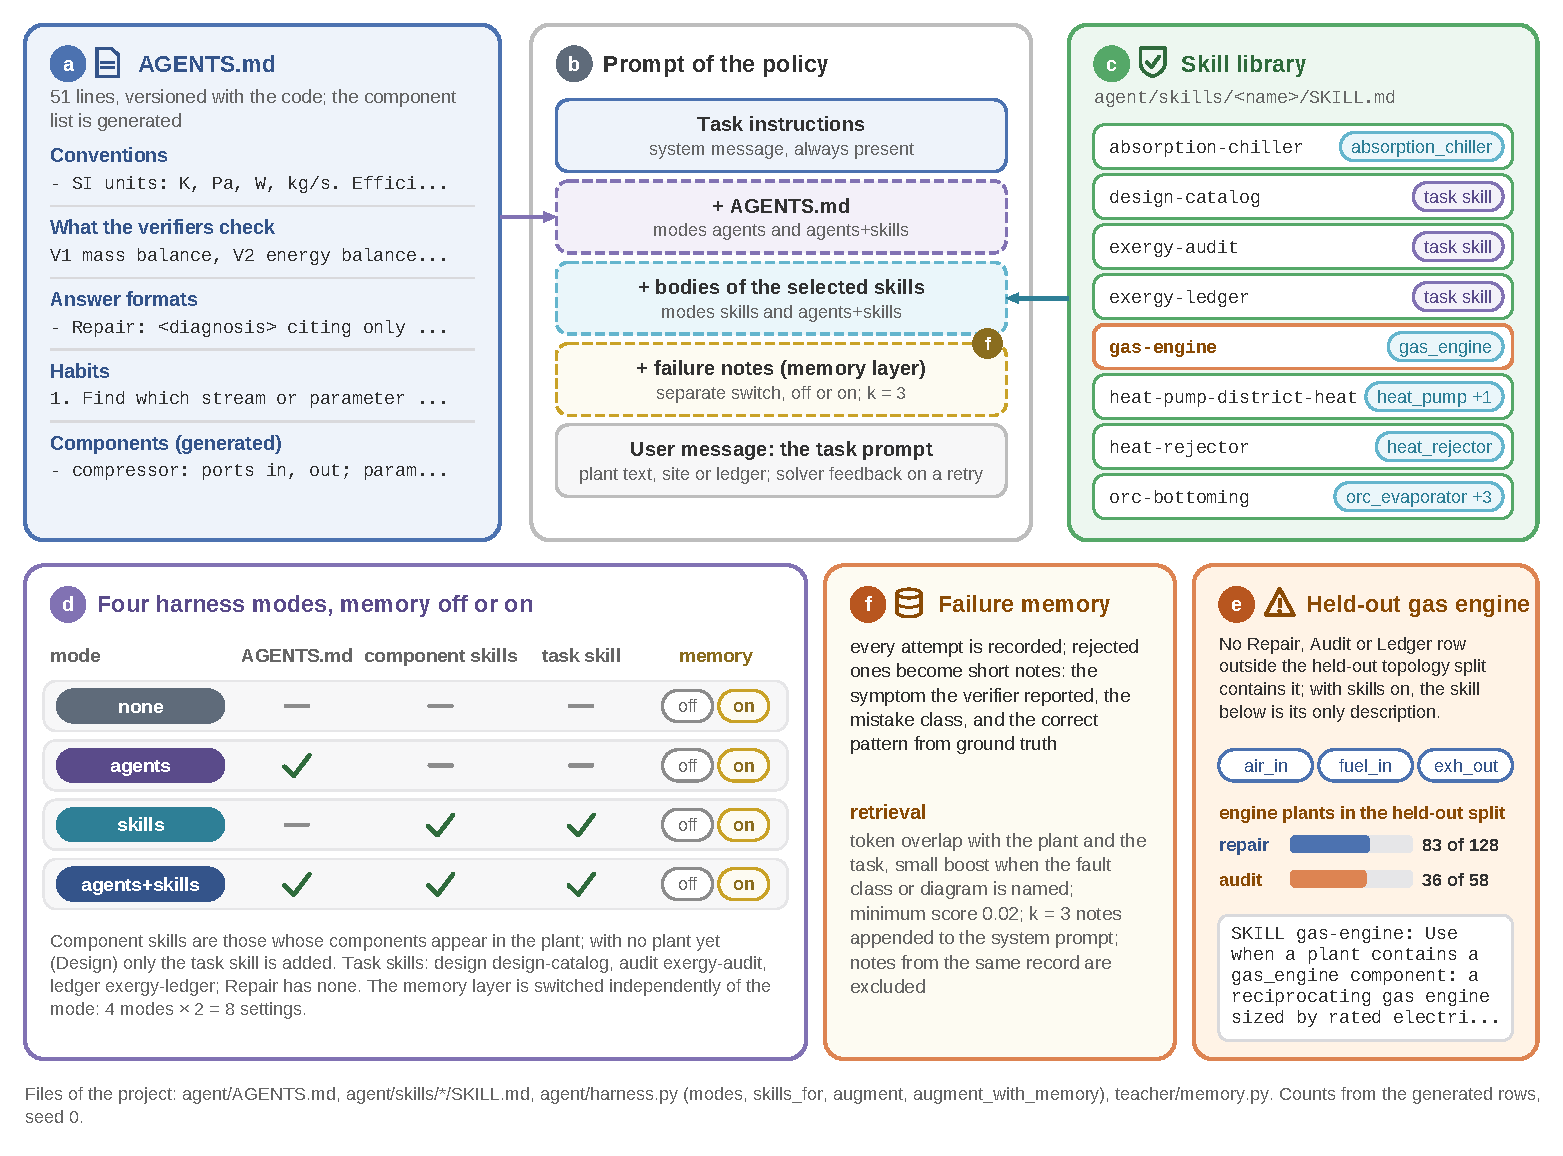
\includegraphics[width=\linewidth]{figures/pdf/fig_harness.pdf}
\caption{Harness and memory. \texttt{AGENTS.md} and the skill library (\val{env.n_skills} skills) are generated from the component registry; four harness modes add none, \texttt{AGENTS.md}, skills or both to the system message, and the memory layer (lexical retrieval of success and failure notes, at most \val{corp.k_memory} notes, notes from the same record excluded) is a separate switch, giving eight settings. With no plant (Design) only the task skill is added. The gas engine is the component held out of training. Data: \texttt{assets/harness.json}, \texttt{assets/corpus.json}.}
\label{fig:fig_harness}
\end{figure}
